
\chapter{누적분포함수}
\label{cumulative}

이번 장에서 사용되는 코드는 {\tt cumulative.py}에 있다.
코드를 다운로드하고 작업하는 것에 대한 정보는 ~\ref{code}을 참조한다.


\section{PMF의 한계점}
\index{PMF}

PMF는 값(value)의 수가 작다면 잘 동작한다. 하지만, 값의 갯수가 증가함에 따라,
각 값과 연관된 확률값이 더 작아지고 확률잡음(random noise)의 효과는 증가한다.

예를 들어, 출산 체중 분포에 관심이 있다고 하자. NSFG 데이터에서 
\verb"totalwgt_lb" 변수가 파운드로 출생 체중을 기록한다.
그림~\ref{nsfg_birthwgt_pmf}이 첫번째 아이와 첫째가 아닌 아이에 대한 체중값을 
PMF로 보여준다.
\index{가족 성장 국가 조사 (National Survey of Family Growth)} 
\index{NSFG} 
\index{출산 체중 (birth weight)}
\index{체중 (weight)!출산 (birth)}

\begin{figure}
% cumulative.py
%\centerline{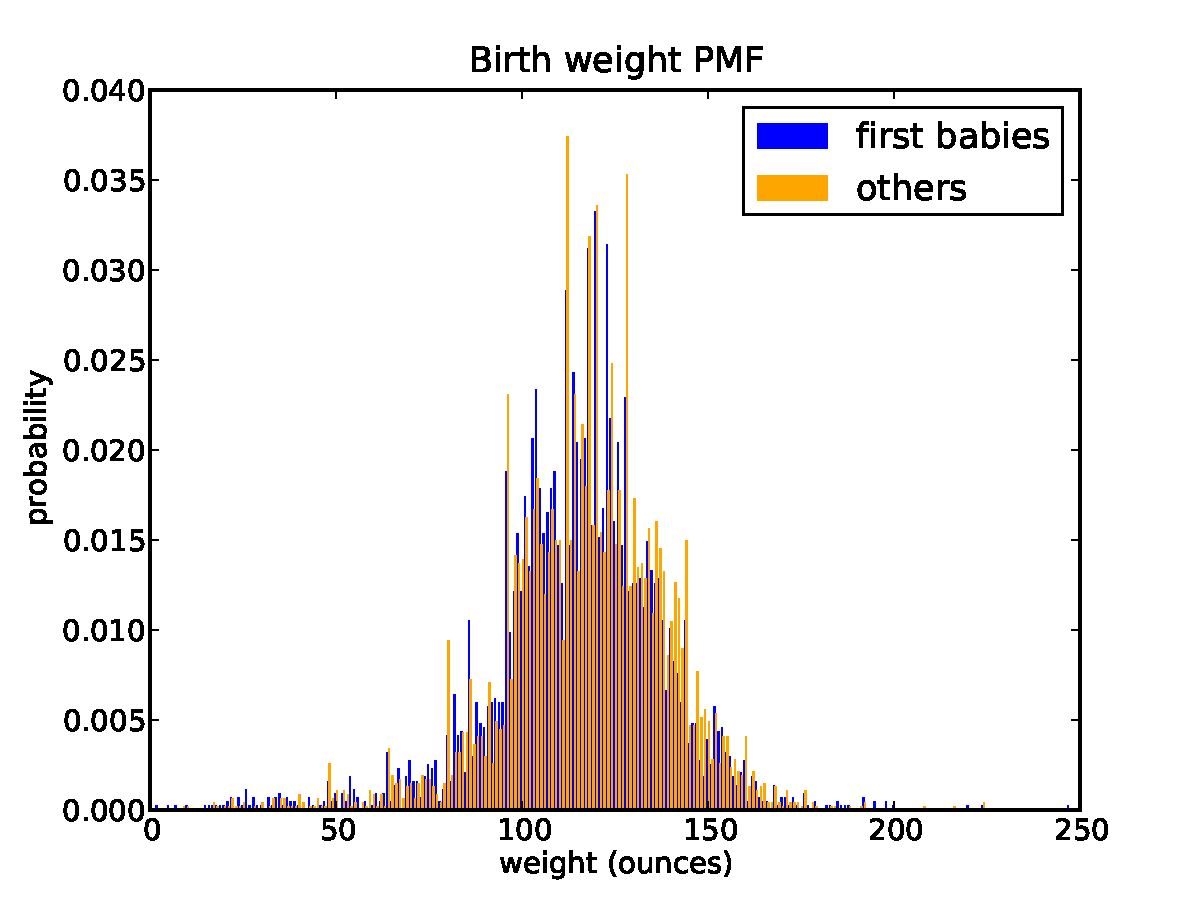
\includegraphics[height=2.5in]{figs/nsfg_birthwgt_pmf.pdf}}
\caption{PMF of birth weights.  This figure shows a limitation
of PMFs: they are hard to compare visually.}
\label{nsfg_birthwgt_pmf}
\end{figure}

전반적으로 분포는 정규분포의 종모양을 닮았다.
평균 근처에 값이 많고 체중이 더 높거나 더 낮아지면 값이 작아진다.

하지만 그림을 이해하기는 어렵다. 뾰족한 것과 골자기가 많고, 두 집단 분포 사이에
명백한 차이도 보인다. 여럿중에서 어느 면이 유의미한지 분간하기는 쉽지 않다.
또한 전반적인 패턴을 보기도 어렵다; 예를 들어, 여러분이 보기에 어느 분포가 평균값이 더 높은가?
\index{통에 담기(binning)}

데이터를 통(bin)에 담아서 이러한 문제는 완화될 수 있다; 즉, 값 범위를 서로 겹쳐지지 않는 구간으로 
나누고 각 통(bin)에 값 갯수를 계수한다. 통에 담는 것(binning)은 유용하지만,
적정한 통크기를 잡는 것은 까다롭다. 잡음을 평활(smooth out)하기 위해서 충분히 큰 통을 잡는 것이 
또한 유용한 정보도 평활할 수도 있다.

이러한 문제를 회피하는 대안이 누적분포함수(cumulative
distribution function, CDF)로 이번 장 학습주제다. 하지만, CDF를 설명하기 전에 백분위수(percentile)를 먼저 설명해야 한다.
\index{CDF}


\section{백분위수 (Percentiles)}
\index{백분위 순위 (percentile rank)}

만약 전국 단위 표준시험을 치르게 되면, 원점수와 {\bf 백분위 순위(percentile rank)} 형태로 시험결과를 받아보게 된다. 이러한 맥락에서 백분위 순위는 시험 당사자보다 적은 점수를 얻는 사람들이 된다.
그래서 만약 ``백분위수 90번째''라면, 시험을 치른 90\% 사람보다 혹은 동등하다는 의미가 된다.

다음에 {\tt scores} 시퀀스 값에서 상대적으로 \verb"your_score" 값에 대한 백분위 순위를 계산하는 방법이 있다.

%
\begin{verbatim}
def PercentileRank(scores, your_score):
    count = 0
    for score in scores:
        if score <= your_score:
            count += 1

    percentile_rank = 100.0 * count / len(scores)
    return percentile_rank
\end{verbatim}

예제로 만약 시퀀스 점수가 55, 66, 77, 88, 99이고, 시험 점수로 88점을 받았다면, 
백분위 순위는 {\tt 100 * 4 / 5}, 80이 된다.

값이 주어진다면, 백분위 순위를 찾기는 쉽다; 반대 방향으로는 다소 더 어렵다.
만약 백분위 순위가 주어진 상태에서 해당하는 값을 찾고자 한다면, 한 선택지는 값을 정렬하고
원하는 값을 찾는 것이다.

%
\begin{verbatim}
def Percentile(scores, percentile_rank):
    scores.sort()
    for score in scores:
        if PercentileRank(scores, score) >= percentile_rank:
            return score
\end{verbatim}

계산 결과는 {\bf 백분위수(percentile)}가 된다. 
예를 들어, 50번째 백분위 수는 백분위 순위가 50 인 값이 된다. 
시험점수 분포에서 50번째 백분위 수는 77이다.
\index{백분위수 (percentile)}

{\tt Percentile} 구현코드가 그다지 효율적이지 않다.
더 나은 접근법은 백분위 순위를 사용해서 해당하는 백분위수 인덱스를 계산하는 것이다.

\begin{verbatim}
def Percentile2(scores, percentile_rank):
    scores.sort()
    index = percentile_rank * (len(scores)-1) // 100
    return scores[index]
\end{verbatim}

``백분위수 (percentile)''와 ``백분위 순위 (percentile rank)'' 차이가 혼동스러울 수 있고
항상 용어를 정확하게 구별하여 사용하지는 않는다. 요약하면,
{\tt PercentileRank} 함수는 값을 인자로 받아 값 집합에서 백분위 순위를 계산한다;
{\tt Percentile} 함수는 백분위 순위를 인자로 받아 해당하는 값을 계산한다. 
\index{백분위 순위 (percentile rank)}

\section{CDF}
\index{CDF}


Now that we understand percentiles and percentile ranks,
we are ready to tackle the {\bf cumulative distribution function}
(CDF).  The CDF is the function that maps from a value to its
percentile rank.
\index{cumulative distribution function}
\index{percentile rank}

The CDF is a function of $x$, where $x$ is any value that might appear
in the distribution.  To evaluate $\CDF(x)$ for a particular value of
$x$, we compute the fraction of values in the distribution less
than or equal to $x$.

Here's what that looks like as a function that takes a sequence,
{\tt sample}, and a value, {\tt x}:
%
\begin{verbatim}
def EvalCdf(sample, x):
    count = 0.0
    for value in sample:
        if value <= x:
            count += 1

    prob = count / len(sample)
    return prob
\end{verbatim}

This function is almost identical to {\tt PercentileRank}, except that
the result is a probability in the range 0--1 rather than a
percentile rank in the range 0--100.
\index{sample}

As an example, suppose we collect a sample with the values 
{\tt [1, 2, 2, 3, 5]}.  Here are some values from its CDF:
%
\[ CDF(0) = 0 \]
%
\[ CDF(1) = 0.2\]
%
\[ CDF(2) = 0.6\]
%
\[ CDF(3) = 0.8\]
%
\[ CDF(4) = 0.8\]
%
\[ CDF(5) = 1\]
%
We can evaluate the CDF for any value of $x$, not just
values that appear in the sample.
If $x$ is less than the smallest value in the sample, $\CDF(x)$ is 0.
If $x$ is greater than the largest value, $\CDF(x)$ is 1.

\begin{figure}
% cumulative.py
%\centerline{\includegraphics[height=2.5in]{figs/cumulative_example_cdf.pdf}}
\caption{Example of a CDF.}
\label{example_cdf}
\end{figure}

Figure~\ref{example_cdf} is a graphical representation of this CDF.
The CDF of a sample is a step function.
\index{step function}


\section{Representing CDFs}
\index{Cdf}

{\tt thinkstats2} provides a class named Cdf that represents
CDFs.  The fundamental methods Cdf provides are:

\begin{itemize}

\item {\tt Prob(x)}: Given a value {\tt x}, computes the probability
  $p = \CDF(x)$.  The bracket operator is equivalent to {\tt Prob}.
\index{bracket operator}

\item {\tt Value(p)}: Given a probability {\tt p}, computes the
corresponding value, {\tt x}; that is, the {\bf inverse CDF} of {\tt p}.
\index{inverse CDF}
\index{CDF, inverse}

\end{itemize}

\begin{figure}
% cumulative.py
%\centerline{\includegraphics[height=2.5in]{figs/cumulative_prglngth_cdf.pdf}}
\caption{CDF of pregnancy length.}
\label{cumulative_prglngth_cdf}
\end{figure}

The Cdf constructor can take as an argument a list of values,
a pandas Series, a Hist, Pmf, or another Cdf.  The following
code makes a Cdf for the distribution of pregnancy lengths in
the NSFG:
\index{NSFG}
\index{pregnancy length}

\begin{verbatim}
    live, firsts, others = first.MakeFrames()
    cdf = thinkstats2.Cdf(live.prglngth, label='prglngth')
\end{verbatim}

{\tt thinkplot} provides a function named {\tt Cdf} that
plots Cdfs as lines:
\index{thinkplot}

\begin{verbatim}
    thinkplot.Cdf(cdf)
    thinkplot.Show(xlabel='weeks', ylabel='CDF')
\end{verbatim}

Figure~\ref{cumulative_prglngth_cdf} shows the result.  One way to
read a CDF is to look up percentiles.  For example, it looks like
about 10\% of pregnancies are shorter than 36 weeks, and about 90\%
are shorter than 41 weeks.  The CDF also provides a visual
representation of the shape of the distribution.  Common values appear
as steep or vertical sections of the CDF; in this example, the mode at
39 weeks is apparent.  There are few values below 30 weeks, so
the CDF in this range is flat.
\index{CDF, interpreting}

It takes some time to get used to CDFs, but once you
do, I think you will find that they show more information, more
clearly, than PMFs.


\section{Comparing CDFs}
\label{birth_weights}
\index{National Survey of Family Growth}
\index{NSFG}
\index{birth weight}
\index{weight!birth}

CDFs are especially useful for comparing distributions.  For
example, here is the code that plots the CDF of birth
weight for first babies and others.
\index{thinkplot}
\index{distributions, comparing}

\begin{verbatim}
    first_cdf = thinkstats2.Cdf(firsts.totalwgt_lb, label='first')
    other_cdf = thinkstats2.Cdf(others.totalwgt_lb, label='other')

    thinkplot.PrePlot(2)
    thinkplot.Cdfs([first_cdf, other_cdf])
    thinkplot.Show(xlabel='weight (pounds)', ylabel='CDF')
\end{verbatim}

\begin{figure}
% cumulative.py
%\centerline{\includegraphics[height=2.5in]{figs/cumulative_birthwgt_cdf.pdf}}
\caption{CDF of birth weights for first babies and others.}
\label{cumulative_birthwgt_cdf}
\end{figure}

Figure~\ref{cumulative_birthwgt_cdf} shows the result.
Compared to Figure~\ref{nsfg_birthwgt_pmf},
this figure makes the shape of the distributions, and the differences
between them, much clearer.  We can see that first babies are slightly
lighter throughout the distribution, with a larger discrepancy above 
the mean.
\index{shape}




\section{Percentile-based statistics}
\index{summary statistic}
\index{interquartile range}
\index{quartile}
\index{percentile}
\index{median}
\index{central tendency}
\index{spread}

Once you have computed a CDF, it is easy to compute percentiles
and percentile ranks.  The Cdf class provides these two methods:
\index{Cdf}
\index{percentile rank}

\begin{itemize}

\item {\tt PercentileRank(x)}: Given a value {\tt x}, computes its
  percentile rank, $100 \cdot \CDF(x)$.

\item {\tt Percentile(p)}: Given a percentile rank {\tt rank},
  computes the corresponding value, {\tt x}.  Equivalent to {\tt
    Value(p/100)}.

\end{itemize}

{\tt Percentile} can be used to compute percentile-based summary
statistics.  For example, the 50th percentile is the value that
divides the distribution in half, also known as the {\bf median}.
Like the mean, the median is a measure of the central tendency
of a distribution.

Actually, there are several definitions of ``median,'' each with
different properties.  But {\tt Percentile(50)} is simple and
efficient to compute.

Another percentile-based statistic is the {\bf interquartile range} (IQR),
which is a measure of the spread of a distribution.  The IQR
is the difference between the 75th and 25th percentiles.

More generally, percentiles are often used to summarize the shape
of a distribution.  For example, the distribution of income is
often reported in ``quintiles''; that is, it is split at the
20th, 40th, 60th and 80th percentiles.  Other distributions
are divided into ten ``deciles''.  Statistics like these that represent
equally-spaced points in a CDF are called {\bf quantiles}.
For more, see \url{https://en.wikipedia.org/wiki/Quantile}.
\index{quantile}
\index{quintile}
\index{decile}



\section{Random numbers}
\label{random}
\index{random number}

Suppose we choose a random sample from the population of live
births and look up the percentile rank of their birth weights.
Now suppose we compute the CDF of the percentile ranks.  What do
you think the distribution will look like?
\index{percentile rank}
\index{birth weight}
\index{weight!birth}

Here's how we can compute it.  First, we make the Cdf of
birth weights:
\index{Cdf}

\begin{verbatim}
    weights = live.totalwgt_lb
    cdf = thinkstats2.Cdf(weights, label='totalwgt_lb')
\end{verbatim}

Then we generate a sample and compute the percentile rank of
each value in the sample.

\begin{verbatim}
    sample = np.random.choice(weights, 100, replace=True)
    ranks = [cdf.PercentileRank(x) for x in sample]
\end{verbatim}

{\tt sample}
is a random sample of 100 birth weights, chosen with {\bf replacement};
that is, the same value could be chosen more than once.  {\tt ranks}
is a list of percentile ranks.
\index{replacement}

Finally we make and plot the Cdf of the percentile ranks.
\index{thinkplot}

\begin{verbatim}
    rank_cdf = thinkstats2.Cdf(ranks)
    thinkplot.Cdf(rank_cdf)
    thinkplot.Show(xlabel='percentile rank', ylabel='CDF')
\end{verbatim}

\begin{figure}
% cumulative.py
%\centerline{\includegraphics[height=2.5in]{figs/cumulative_random.pdf}}
\caption{CDF of percentile ranks for a random sample of birth weights.}
\label{cumulative_random}
\end{figure}

Figure~\ref{cumulative_random} shows the result.  The CDF is
approximately a straight line, which means that the distribution
is uniform.

That outcome might be non-obvious, but it is a consequence of
the way the CDF is defined.  What this figure shows is that 10\%
of the sample is below the 10th percentile, 20\% is below the
20th percentile, and so on, exactly as we should expect.

So, regardless of the shape of the CDF, the distribution of
percentile ranks is uniform.  This property is useful, because it
is the basis of a simple and efficient algorithm for generating
random numbers with a given CDF.  Here's how:
\index{inverse CDF algorithm}
\index{random number}

\begin{itemize}

\item Choose a percentile rank uniformly from the range 0--100.

\item Use {\tt Cdf.Percentile} to find the value in the distribution
that corresponds to the percentile rank you chose.
\index{Cdf}

\end{itemize}

Cdf provides an implementation of this algorithm, called
{\tt Random}:

\begin{verbatim}
# class Cdf:
    def Random(self):
        return self.Percentile(random.uniform(0, 100))
\end{verbatim}

Cdf also provides {\tt Sample}, which takes an integer,
{\tt n}, and returns a list of {\tt n} values chosen at random
from the Cdf.


\section{Comparing percentile ranks}

Percentile ranks are useful for comparing measurements across
different groups.  For example, people who compete in foot races are
usually grouped by age and gender.  To compare people in different
age groups, you can convert race times to percentile ranks.
\index{percentile rank}

A few years ago I ran the James Joyce Ramble 10K in
Dedham MA; I finished in 42:44, which was 97th in a field of 1633.  I beat or
tied 1537 runners out of 1633, so my percentile rank in the field is
94\%.  \index{James Joyce Ramble} \index{race time}

More generally, given position and field size, we can compute
percentile rank:
\index{field size}

\begin{verbatim}
def PositionToPercentile(position, field_size):
    beat = field_size - position + 1
    percentile = 100.0 * beat / field_size
    return percentile
\end{verbatim}

In my age group, denoted M4049 for ``male between 40 and 49 years of
age'', I came in 26th out of 256.  So my percentile rank in my age
group was 90\%.
\index{age group}

If I am still running in 10 years (and I hope I am), I will be in
the M5059 division.  Assuming that my percentile rank in my division
is the same, how much slower should I expect to be?

I can answer that question by converting my percentile rank in M4049
to a position in M5059.  Here's the code:

\begin{verbatim}
def PercentileToPosition(percentile, field_size):
    beat = percentile * field_size / 100.0
    position = field_size - beat + 1
    return position
\end{verbatim}

There were 171 people in M5059, so I would have to come in between
17th and 18th place to have the same percentile rank.  The finishing
time of the 17th runner in M5059 was 46:05, so that's the time I will
have to beat to maintain my percentile rank.


\section{Exercises}

For the following exercises, you can start with \verb"chap04ex.ipynb".
My solution is in \verb"chap04soln.ipynb".

\begin{exercise}
How much did you weigh at birth?  If you don't know, call your mother
or someone else who knows.  Using the NSFG data (all live births),
compute the distribution of birth weights and use it to find your
percentile rank.  If you were a first baby, find your percentile rank
in the distribution for first babies.  Otherwise use the distribution
for others.  If you are in the 90th percentile or higher, call your
mother back and apologize.
\index{birth weight}
\index{weight!birth}

\end{exercise}

\begin{exercise}
The numbers generated by {\tt random.random} are supposed to be
uniform between 0 and 1; that is, every value in the range
should have the same probability.

Generate 1000 numbers from {\tt random.random} and plot their
PMF and CDF.  Is the distribution uniform?
\index{uniform distribution}
\index{distribution!uniform}
\index{random number}

\end{exercise}


\section{Glossary}

\begin{itemize}

\item percentile rank: The percentage of values in a distribution that are
less than or equal to a given value.
\index{percentile rank}

\item percentile: The value associated with a given percentile rank.
\index{percentile}

\item cumulative distribution function (CDF): A function that maps
  from values to their cumulative probabilities.  $\CDF(x)$ is the
  fraction of the sample less than or equal to $x$.  \index{CDF}
\index{cumulative probability}

\item inverse CDF: A function that maps from a cumulative probability,
  $p$, to the corresponding value.
\index{inverse CDF}
\index{CDF, inverse}

\item median: The 50th percentile, often used as a measure of central
  tendency.  \index{median}

\item interquartile range: The difference between
the 75th and 25th percentiles, used as a measure of spread.
\index{interquartile range}

\item quantile: A sequence of values that correspond to equally spaced
percentile ranks; for example, the quartiles of a distribution are
the 25th, 50th and 75th percentiles.
\index{quantile}

\item replacement: A property of a sampling process. ``With replacement''
means that the same value can be chosen more than once; ``without
replacement'' means that once a value is chosen, it is removed from
the population.
\index{replacement}

\end{itemize}

